\documentclass{beamer}

\mode<presentation>
\usepackage{amsmath,amssymb,mathtools}
\usepackage{textcomp}
\usepackage{gensymb}
\usepackage{adjustbox}
\usepackage{subcaption}
\usepackage{enumitem}
\usepackage[utf8]{inputenc}
\usepackage{amssymb}
\usepackage{newunicodechar}
\usepackage{enumitem}
\setlist{nosep} % optional: removes vertical gaps
\setlist[enumerate]{label=\arabic*)} % custom numbering if you want

\newunicodechar{√}{$\sqrt{\;}$}
\newunicodechar{✅}{\checkmark}
\newunicodechar{❌}{\texttimes}
\usepackage{multicol}
\usepackage{listings}
\usepackage{url}
\usepackage{graphicx} % <-- needed for images
\def\UrlBreaks{\do\/\do-}

\usetheme{Boadilla}
\usecolortheme{lily}
\setbeamertemplate{footline}{
  \leavevmode%
  \hbox{%
  \begin{beamercolorbox}[wd=\paperwidth,ht=2ex,dp=1ex,right]{author in head/foot}%
    \insertframenumber{} / \inserttotalframenumber\hspace*{2ex}
  \end{beamercolorbox}}%
  \vskip0pt%
}
\setbeamertemplate{navigation symbols}{}

\lstset{
  frame=single,
  breaklines=true,
  columns=fullflexible,
  basicstyle=\ttfamily\tiny   % tiny font so code fits
}

\numberwithin{equation}{section}

% ---- your macros ----
\providecommand{\nCr}[2]{\,^{#1}{#2}}
\providecommand{\nPr}[2]{\,^{#1}P_{#2}}
\providecommand{\mbf}{\mathbf}
\providecommand{\pr}[1]{\ensuremath{\Pr\left(#1\right)}}
\providecommand{\qfunc}[1]{\ensuremath{Q\left(#1\right)}}
\providecommand{\sbrak}[1]{\ensuremath{{}\left[#1\right]}}
\providecommand{\lsbrak}[1]{\ensuremath{{}\left[#1\right.}}
\providecommand{\rsbrak}[1]{\ensuremath{\left.#1\right]}}
\providecommand{\brak}[1]{\ensuremath{\left(#1\right)}}
\providecommand{\lbrak}[1]{\ensuremath{\left(#1\right.}}
\providecommand{\rbrak}[1]{\ensuremath{\left.#1\right)}}
\providecommand{\cbrak}[1]{\ensuremath{\left\{#1\right\}}}
\providecommand{\lcbrak}[1]{\ensuremath{\left\{#1\right.}}
\providecommand{\rcbrak}[1]{\ensuremath{\left.#1\right\}}}
\theoremstyle{remark}
\newtheorem{rem}{Remark}
\newcommand{\sgn}{\mathop{\mathrm{sgn}}}
\providecommand{\abs}[1]{\left\vert#1\right\vert}
\providecommand{\res}[1]{\Res\displaylimits_{#1}}
\providecommand{\norm}[1]{\lVert#1\rVert}
\providecommand{\mtx}[1]{\mathbf{#1}}
\providecommand{\mean}[1]{E\left[ #1 \right]}
\providecommand{\fourier}{\overset{\mathcal{F}}{ \rightleftharpoons}}
\providecommand{\system}{\overset{\mathcal{H}}{ \longleftrightarrow}}
\providecommand{\dec}[2]{\ensuremath{\overset{#1}{\underset{#2}{\gtrless}}}}
\newcommand{\myvec}[1]{\ensuremath{\begin{pmatrix}#1\end{pmatrix}}}
\let\vec\mathbf
% ---------------------

\title{Matgeo Presentation - Problem 2.7.33}
\author{ee25btech11021 - Dhanush sagar}

\begin{document}
	

		




%---------------- Title Page ----------------
\begin{frame}
  \titlepage
\end{frame}

%---------------- Problem Statement ----------------
\begin{frame}{Problem Statement}
Find the equation of the plane containing the two parallel lines 
$\frac{x-1}{2} = \frac{y+1}{-1} = \frac{z}{3}$ and 
$\frac{x}{4} = \frac{y-2}{-2} = \frac{z+1}{6}$. 
Also, determine whether the plane thus obtained contains the line 
$\frac{x-2}{3} = \frac{y-1}{1} = \frac{z-2}{5}$.\\
\end{frame}

%---------------- Mathematical Formula ----------------
\begin{frame}{solution}

The general equation of a plane is
\begin{align}
\vec{n}^\top \vec{X} &= c
\end{align}
where $\vec{n}$ is the normal vector.

\noindent
\begin{align}
\text{Line 1: } & \frac{x-1}{2} = \frac{y+1}{-1} = \frac{z}{3} \\
\text{Line 2: } & \frac{x}{4} = \frac{y-2}{-2} = \frac{z+1}{6}
\end{align}
From the two given parallel lines we extract:
\begin{align}
\vec{v} &= \myvec{2\\-1\\3} 
&& \text{(common direction vector)} \\
\vec{p}_1 &= \myvec{1\\-1\\0}, \quad 
\vec{p}_2 = \myvec{0\\2\\-1} 
&& \text{(points on each line)} 
\end{align}
\end{frame}
\begin{frame}{solution}
\begin{align}
\vec{d} &= \vec{p}_2 - \vec{p}_1 = \myvec{-1\\3\\-1}
&& \text{(difference of points)}
\end{align}

\noindent
The normal $\vec{n}$ must be orthogonal to both $\vec{v}$ and $\vec{d}$:
\begin{align}
\vec{n}^\top \vec{v} &= 0 \\
\vec{n}^\top \vec{d} &= 0
\end{align}

\noindent
To fix the scale of $\vec{n}$, we impose a normalization condition using point $\vec{p}_1$:
\begin{align}
\vec{n}^\top \vec{p}_1 &= 1
\end{align}

\noindent
Put these column vectors into rows of new matrix $\vec{A}$
\begin{align}
\vec{A} = \myvec{2 & -1 & 3 \\ -1 & 3 & -1 \\ 1 & -1 & 0}
\end{align}
\end{frame}
\begin{frame}{solution}
from the equations 0.7,0.8,0.9 we can write 
\begin{align}
\myvec{2 & -1 & 3 \\ -1 & 3 & -1 \\ 1 & -1 & 0}\vec{n}
&= \myvec{0 \\ 0 \\ 1}
\end{align}

\noindent
This augmented matrix form is
\begin{align}
\myvec{2 & -1 & 3 & 0 \\ -1 & 3 & -1 & 0 \\ 1 & -1 & 0 & 1}
\end{align}

\noindent
Row-reducing:
\begin{align}
\myvec{2 & -1 & 3 & 0 \\ -1 & 3 & -1 & 0 \\ 1 & -1 & 0 & 1}
&\xrightarrow{R_2 \to 2R_2+R_1}
\myvec{2 & -1 & 3 & 0 \\ 0 & 5 & 1 & 0 \\ 1 & -1 & 0 & 1} \\[6pt]
&\xrightarrow{R_3 \to R_3 - \tfrac{1}{2}R_1}
\myvec{2 & -1 & 3 & 0 \\ 0 & 5 & 1 & 0 \\ 0 & -\tfrac{1}{2} & -\tfrac{3}{2} & 1} 
\end{align}
\end{frame}
\begin{frame}{solution}
\begin{align}
&\xrightarrow{R_3 \to 5R_3 - R_2}
\myvec{2 & -1 & 3 & 0 \\ 0 & 5 & 1 & 0 \\ 0 & 0 & -7 & 5}
\end{align}

\noindent
From the last row, the third entry of $\vec{n}$ is $-\tfrac{5}{7}$.  
Back-substitution gives
\begin{align}
\vec{n} &= \myvec{\tfrac{8}{7} \\[4pt] \tfrac{1}{7} \\[4pt] -\tfrac{5}{7}}
\end{align}

\noindent
Therefore, the plane equation is
\begin{align}
\vec{n}^\top \vec{X} &= 1
\end{align}

\noindent
Equivalently, multiplying throughout by $7$ gives
\begin{align}
\myvec{8 & 1 & -5}\vec{X} &= 7
\end{align}

\noindent
This is the required plane passing through the given parallel lines.
\end{frame}
\begin{frame}{solution}

\noindent Check if the third line $\frac{x-2}{3} = \frac{y-1}{1} = \frac{z-2}{5}$. lies in the plane by verifying the point and direction:
\begin{align}
\vec{P}_3 = \myvec{2\\1\\2}, \quad \vec{d}_3 = \myvec{3\\1\\5} \\
\vec{n}^T \vec{P}_3 = \myvec{8 & 1 & -5}\myvec{2\\1\\2} = 7 \\
\vec{n}^T \vec{d}_3 = \myvec{8 & 1 & -5}\myvec{3\\1\\5} = 0
\end{align}

\noindent Therefore, the plane containing the first two lines has the matrix form:
\[
\myvec{8 & 1 & -5}\,\vec{r} = 7
\]  
and it also contains the third line.
\end{frame}



%---------------- C Source Code ----------------
\begin{frame}[fragile]{C Source Code:line data.c}
\begin{verbatim}
#include <stdio.h>
typedef struct {
    double x, y, z;
} Vec3;
// Function to return points and direction vectors for lines
void get_lines(Vec3* P1, Vec3* d1, Vec3* P2, Vec3* d2, Vec3* P3, Vec3* d3) {
    // Line 1
    P1->x = 1; P1->y = -1; P1->z = 0;
    d1->x = 2; d1->y = -1; d1->z = 3;
    // Line 2
    P2->x = 0; P2->y = 2; P2->z = -1;
    d2->x = 4; d2->y = -2; d2->z = 6;
    // Line 3
    P3->x = 2; P3->y = 1; P3->z = 2;
    d3->x = 3; d3->y = 1; d3->z = 5;
}
\end{verbatim}
\end{frame}

%---------------- Python solve.py ----------------
\begin{frame}[fragile]{Python Script:plane solver.py}
\begin{verbatim}
import ctypes
import numpy as np
# Load shared library
lib = ctypes.CDLL("./libline_data.so")
# Define Vec3 struct
class Vec3(ctypes.Structure):
    _fields_ = [("x", ctypes.c_double),
                ("y", ctypes.c_double),
                ("z", ctypes.c_double)]
# Create instances
P1 = Vec3(); d1 = Vec3()
P2 = Vec3(); d2 = Vec3()
P3 = Vec3(); d3 = Vec3()
# Populate points and directions
lib.get_lines(ctypes.byref(P1), ctypes.byref(d1), ctypes.byref(P2), ctypes.byref(d2), ctypes.byref(P3), ctypes.byref(d3))
\end{verbatim}
\end{frame}
\begin{frame}[fragile]{Python Script:plane solver.py}
\begin{verbatim}
# Convert to numpy arrays
P1 = np.array([P1.x, P1.y, P1.z])
d1 = np.array([d1.x, d1.y, d1.z])
P2 = np.array([P2.x, P2.y, P2.z])
d2 = np.array([d2.x, d2.y, d2.z])
P3 = np.array([P3.x, P3.y, P3.z])
d3 = np.array([d3.x, d3.y, d3.z])
# Vector between points on first two lines
v = P2 - P1
# Constraint matrix
A = np.array([d1, v])
# Null space to find plane normal
U, S, Vt = np.linalg.svd(A)
n = Vt.T[:, -1]
# Scale normal for simplicity
n = n / n[-1]
\end{verbatim}
\end{frame}
\begin{frame}[fragile]{Python Script:plane solver.py}
\begin{verbatim}
# Plane equation: n . r = n . P1
d_plane = np.dot(n, P1)
print("Plane normal:", n)
print("Plane equation: {}*x + {}*y + {}*z = {}".format(n[0], n[1], n[2], d_plane))
# Check if third line lies on plane
dot_point = np.dot(n, P3) - d_plane
dot_dir = np.dot(n, d3)
if abs(dot_point) < 1e-6 and abs(dot_dir) < 1e-6:
    print("Line 3 lies on the plane")
else:
    print("Line 3 does NOT lie on the plane")

\end{verbatim}
\end{frame}
\begin{frame}[fragile]{Python Script: plot lines plane.py}
\begin{verbatim}
import matplotlib.pyplot as plt
from mpl_toolkits.mplot3d import Axes3D
import numpy as np
from plane_solver import P1, d1, P2, d2, P3, d3, n, d_plane  # reuse computed values
points = [P1, P2, P3]
directions = [d1, d2, d3]
fig = plt.figure()
ax = fig.add_subplot(111, projection='3d')
# Plot lines
t = np.linspace(-1, 2, 50)
for i, (P, d) in enumerate(zip(points, directions)):
    X = P[0] + d[0]*t
    Y = P[1] + d[1]*t
    Z = P[2] + d[2]*t
    ax.plot(X, Y, Z, label=f'Line {i+1}')
    ax.scatter(P[0], P[1], P[2], s=50)
    ax.text(P[0], P[1], P[2], f'P{i+1}({P[0]},{P[1]},{P[2]})')
\end{verbatim}
\end{frame}
\begin{frame}[fragile]{Python Script: plot lines plane.py}
\begin{verbatim}
# Plot plane
xx, yy = np.meshgrid(np.linspace(-1,3,10), np.linspace(-1,3,10))
zz = (d_plane - n[0]*xx - n[1]*yy)/n[2]
ax.plot_surface(xx, yy, zz, alpha=0.3, color='cyan')

ax.set_xlabel('X')
ax.set_ylabel('Y')
ax.set_zlabel('Z')
ax.legend()
plt.savefig("lines_and_plane.png", dpi=300, bbox_inches='tight')
plt.show()
\end{verbatim}
\end{frame}

%---------------- Result Plot ----------------
\begin{frame}{Result Plot}
 \begin{figure}[H]
     \centering
     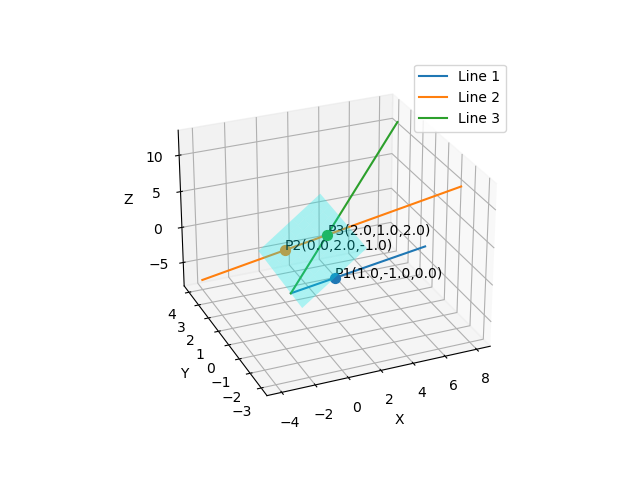
\includegraphics[width=0.7\columnwidth]{figs/fig1.png}
     \caption*{}
     \label{fig:fig1}
 \end{figure}
 
\end{frame}

\end{document}
\end{document}
